% inspired by https://github.com/tonyelhabr/cheat-sheet-rmarkdown/blob/master/template.tex
% adjusted by Issac Lee (https://github.com/issactoast)
% distributed by Statistics playbook (https://github.com/statisticsplaybook)
% last modified in Mar 2, 2021

\documentclass[10pt,quotespacing]{oblivoir}

% Package imports.
\usepackage{fapapersize}
\usepackage{kotex}
\usepackage{multicol}
\usepackage{calc}
\usepackage{amsmath,amsthm,amsfonts,amssymb}
\usepackage{color,graphicx,overpic}
\usepackage{hyperref}
\usepackage[utf8]{inputenc}
\usepackage{textcomp} % provide euro and other symbols
\usepackage{setspace}\singlespacing
\usepackage{tikz}
\usepackage[most]{tcolorbox}
\tcbuselibrary{skins,breakable}

\usepackage{color}
\usepackage{fancyvrb}
\newcommand{\VerbBar}{|}
\newcommand{\VERB}{\Verb[commandchars=\\\{\}]}
\DefineVerbatimEnvironment{Highlighting}{Verbatim}{commandchars=\\\{\}}
% Add ',fontsize=\small' for more characters per line
\usepackage{framed}
\definecolor{shadecolor}{RGB}{248,248,248}
\newenvironment{Shaded}{\begin{snugshade}}{\end{snugshade}}
\newcommand{\AlertTok}[1]{\textcolor[rgb]{0.94,0.16,0.16}{#1}}
\newcommand{\AnnotationTok}[1]{\textcolor[rgb]{0.56,0.35,0.01}{\textbf{\textit{#1}}}}
\newcommand{\AttributeTok}[1]{\textcolor[rgb]{0.77,0.63,0.00}{#1}}
\newcommand{\BaseNTok}[1]{\textcolor[rgb]{0.00,0.00,0.81}{#1}}
\newcommand{\BuiltInTok}[1]{#1}
\newcommand{\CharTok}[1]{\textcolor[rgb]{0.31,0.60,0.02}{#1}}
\newcommand{\CommentTok}[1]{\textcolor[rgb]{0.56,0.35,0.01}{\textit{#1}}}
\newcommand{\CommentVarTok}[1]{\textcolor[rgb]{0.56,0.35,0.01}{\textbf{\textit{#1}}}}
\newcommand{\ConstantTok}[1]{\textcolor[rgb]{0.00,0.00,0.00}{#1}}
\newcommand{\ControlFlowTok}[1]{\textcolor[rgb]{0.13,0.29,0.53}{\textbf{#1}}}
\newcommand{\DataTypeTok}[1]{\textcolor[rgb]{0.13,0.29,0.53}{#1}}
\newcommand{\DecValTok}[1]{\textcolor[rgb]{0.00,0.00,0.81}{#1}}
\newcommand{\DocumentationTok}[1]{\textcolor[rgb]{0.56,0.35,0.01}{\textbf{\textit{#1}}}}
\newcommand{\ErrorTok}[1]{\textcolor[rgb]{0.64,0.00,0.00}{\textbf{#1}}}
\newcommand{\ExtensionTok}[1]{#1}
\newcommand{\FloatTok}[1]{\textcolor[rgb]{0.00,0.00,0.81}{#1}}
\newcommand{\FunctionTok}[1]{\textcolor[rgb]{0.00,0.00,0.00}{#1}}
\newcommand{\ImportTok}[1]{#1}
\newcommand{\InformationTok}[1]{\textcolor[rgb]{0.56,0.35,0.01}{\textbf{\textit{#1}}}}
\newcommand{\KeywordTok}[1]{\textcolor[rgb]{0.13,0.29,0.53}{\textbf{#1}}}
\newcommand{\NormalTok}[1]{#1}
\newcommand{\OperatorTok}[1]{\textcolor[rgb]{0.81,0.36,0.00}{\textbf{#1}}}
\newcommand{\OtherTok}[1]{\textcolor[rgb]{0.56,0.35,0.01}{#1}}
\newcommand{\PreprocessorTok}[1]{\textcolor[rgb]{0.56,0.35,0.01}{\textit{#1}}}
\newcommand{\RegionMarkerTok}[1]{#1}
\newcommand{\SpecialCharTok}[1]{\textcolor[rgb]{0.00,0.00,0.00}{#1}}
\newcommand{\SpecialStringTok}[1]{\textcolor[rgb]{0.31,0.60,0.02}{#1}}
\newcommand{\StringTok}[1]{\textcolor[rgb]{0.31,0.60,0.02}{#1}}
\newcommand{\VariableTok}[1]{\textcolor[rgb]{0.00,0.00,0.00}{#1}}
\newcommand{\VerbatimStringTok}[1]{\textcolor[rgb]{0.31,0.60,0.02}{#1}}
\newcommand{\WarningTok}[1]{\textcolor[rgb]{0.56,0.35,0.01}{\textbf{\textit{#1}}}}

  \setmainfont[]{NanumMyeongjo}

% 편집용지(가로), 편집용지(세로), 왼,오른,위,아래
\usefapapersize{257mm, 188mm, 5mm, 5mm, 5mm, 5mm}

\hypersetup{
    colorlinks=true,
    linkcolor=blue,
    filecolor=magenta,      
    urlcolor=black,
}

\pagestyle{empty}

% No section numbers.
\setcounter{secnumdepth}{0}

% Minimal paragraph indenting and spacing.
\setlength{\parindent}{0pt}
\setlength{\parskip}{0pt plus 0.5ex}
\setlength{\OuterFrameSep}{-0.1pt}

% Define colorboxes
\newcommand{\bcolorbox}{\begin{tcolorbox}[width=\linewidth, enhanced, breakable,colback=white,colframe=cyan!50!black]}
\newcommand{\ecolorbox}{\end{tcolorbox}}

% Redefine \section
\makeatletter
\preto{\@verbatim}{\topsep=0pt \partopsep=0pt}
\renewcommand{\section}{\@startsection{section}{1}{0mm}%
                        {1ex plus -.5ex minus -.2ex}%
                        {0.5\baselineskip}%
                        {\normalfont\scriptsize\bfseries}}
\makeatother

% Boarder line
% code steal from stack over flow
% https://tex.stackexchange.com/questions/801/what-is-the-easiest-way-to-get-borders-around-a-page-in-latex
\usepackage{pgf}
\usepackage{pgfpages}

\pgfpagesdeclarelayout{boxed}
{
  \edef\pgfpageoptionborder{0pt}
}
{
  \pgfpagesphysicalpageoptions
  {%
    logical pages=1,%
  }
  \pgfpageslogicalpageoptions{1}
  {
    border code=\pgfsetlinewidth{2pt}\pgfsetstrokecolor{black!75!cyan}\pgfstroke,%
    border shrink=\pgfpageoptionborder,%
    resized width=.95\pgfphysicalwidth,%
    resized height=.95\pgfphysicalheight,%
    center=\pgfpoint{.5\pgfphysicalwidth}{.5\pgfphysicalheight}%
  }%
}

\pgfpagesuselayout{boxed}

\begin{document}

\textbf{example} Cheatsheet  by \textbf{Issac Lee}

% ncol pandoc parameter
\begin{multicols*}{4}


% Can play around with these as desired.
\setlength{\premulticols}{0.25pt}
\setlength{\postmulticols}{0.25pt}
\setlength{\multicolsep}{0.25pt}
\setlength{\columnsep}{0.25pt}

% This is the "magic" pandoc variable. (This is where your Rmarkdown document is inserted.)
%\tiny
\scriptsize

\bcolorbox

\hypertarget{reduce-and-accumulate-uxd568uxc218}{%
\section{\texorpdfstring{\textbf{\texttt{reduce} and \texttt{accumulate} 함수}}{reduce and accumulate 함수}}\label{reduce-and-accumulate-uxd568uxc218}}

Lorem ipsum dolor sit amet, consectetur adipiscing elit, sed do eiusmod tempor incididunt ut labore et dolore magna aliqua. Ut enim ad minim veniam, quis nostrud exercitation ullamco laboris nisi ut aliquip ex ea commodo consequat.

\begin{Shaded}
\begin{Highlighting}[]
\FunctionTok{reduce}\NormalTok{(}\DecValTok{1}\SpecialCharTok{:}\DecValTok{10}\NormalTok{, sum)}
\end{Highlighting}
\end{Shaded}

\begin{verbatim}
>> [1] 55
\end{verbatim}

\begin{Shaded}
\begin{Highlighting}[]
\FunctionTok{accumulate}\NormalTok{(}\DecValTok{1}\SpecialCharTok{:}\DecValTok{10}\NormalTok{, sum)}
\end{Highlighting}
\end{Shaded}

\begin{verbatim}
>>  [1]  1  3  6 10 15 21 28 36 45 55
\end{verbatim}

\ecolorbox

Lorem ipsum dolor sit amet, consectetur adipiscing elit, sed do eiusmod tempor incididunt ut labore et dolore magna aliqua. Ut enim ad minim veniam, quis nostrud exercitation ullamco laboris nisi ut aliquip ex ea commodo consequat. Duis aute irure dolor in reprehenderit in voluptate velit esse cillum dolore eu fugiat nulla pariatur. Excepteur sint occaecat cupidatat non proident, sunt in culpa qui officia deserunt mollit anim id est laborum.

\begin{equation}
\begin{aligned} 
X \sim \mathcal{N}(\mu, \sigma^2) &= 1steqr \\
2ndeql &= 2ndeqr
\end{aligned}
\label{eq:tag}
\end{equation}

\bcolorbox

\hypertarget{reduce-uxd568uxc218-uxc751uxc6a9-1}{%
\section{\texorpdfstring{\texttt{reduce} 함수 응용 1}{reduce 함수 응용 1}}\label{reduce-uxd568uxc218-uxc751uxc6a9-1}}

이것이야말로 그들을 황금시대를 우는 풀이 시들어 청춘 속에 말이다. 이상의 구하지 사랑의 그들은 현저하게 따뜻한 피다. 이상의 붙잡아 속에서 피다. 보배를 품에 용

\begin{Shaded}
\begin{Highlighting}[]
\NormalTok{paste2 }\OtherTok{\textless{}{-}} \ControlFlowTok{function}\NormalTok{(x, y, }\AttributeTok{sep =} \StringTok{"."}\NormalTok{)\{}
  \FunctionTok{paste}\NormalTok{(x, y, }\AttributeTok{sep =}\NormalTok{ sep)}
\NormalTok{\}}
\NormalTok{letters[}\DecValTok{1}\SpecialCharTok{:}\DecValTok{4}\NormalTok{] }\SpecialCharTok{\%\textgreater{}\%} \FunctionTok{reduce}\NormalTok{(paste2)}
\end{Highlighting}
\end{Shaded}

\begin{verbatim}
>> [1] "a.b.c.d"
\end{verbatim}

\ecolorbox

Lorem ipsum dolor sit amet, consectetur adipiscing elit, sed do eiusmod tempor incididunt ut labore et dolore magna aliqua. Ut enim ad minim veniam, quis nostrud exercitation ullamco laboris nisi ut aliquip ex ea commodo consequat. Duis aute irure dolor in reprehenderit in voluptate velit esse cillum dolore eu fugiat nulla pariatur. Excepteur sint occaecat cupidatat non proident, sunt in culpa qui officia deserunt mollit anim id est laborum.

\bcolorbox

\hypertarget{reduce-uxd568uxc218-uxc751uxc6a9-2}{%
\section{\texorpdfstring{\texttt{reduce} 함수 응용 2}{reduce 함수 응용 2}}\label{reduce-uxd568uxc218-uxc751uxc6a9-2}}

이것이야말로 그들을 황금시대를 우는 풀이 시들어 청춘 속에 말이다. 이상의 구하지 사랑의 그들은 현저하게 따뜻한 피다. 이상의 붙잡아 속에서 피다. 보배를 품에 용

\begin{Shaded}
\begin{Highlighting}[]
\NormalTok{paste2 }\OtherTok{\textless{}{-}} \ControlFlowTok{function}\NormalTok{(x, y, }\AttributeTok{sep =} \StringTok{"."}\NormalTok{)\{}
  \FunctionTok{paste}\NormalTok{(x, y, }\AttributeTok{sep =}\NormalTok{ sep)}
\NormalTok{\}}
\NormalTok{letters[}\DecValTok{1}\SpecialCharTok{:}\DecValTok{4}\NormalTok{] }\SpecialCharTok{\%\textgreater{}\%} \FunctionTok{reduce}\NormalTok{(paste2)}
\end{Highlighting}
\end{Shaded}

\begin{verbatim}
>> [1] "a.b.c.d"
\end{verbatim}

\ecolorbox
\bcolorbox

\hypertarget{reduce-uxd568uxc218-uxc751uxc6a9-3}{%
\section{\texorpdfstring{\texttt{reduce} 함수 응용 3}{reduce 함수 응용 3}}\label{reduce-uxd568uxc218-uxc751uxc6a9-3}}

test plot

\begin{Shaded}
\begin{Highlighting}[]
\NormalTok{x }\OtherTok{\textless{}{-}} \DecValTok{1}\SpecialCharTok{:}\DecValTok{10}
\NormalTok{y }\OtherTok{\textless{}{-}} \FunctionTok{sqrt}\NormalTok{(x)}
\FunctionTok{plot}\NormalTok{(x, y)}
\end{Highlighting}
\end{Shaded}

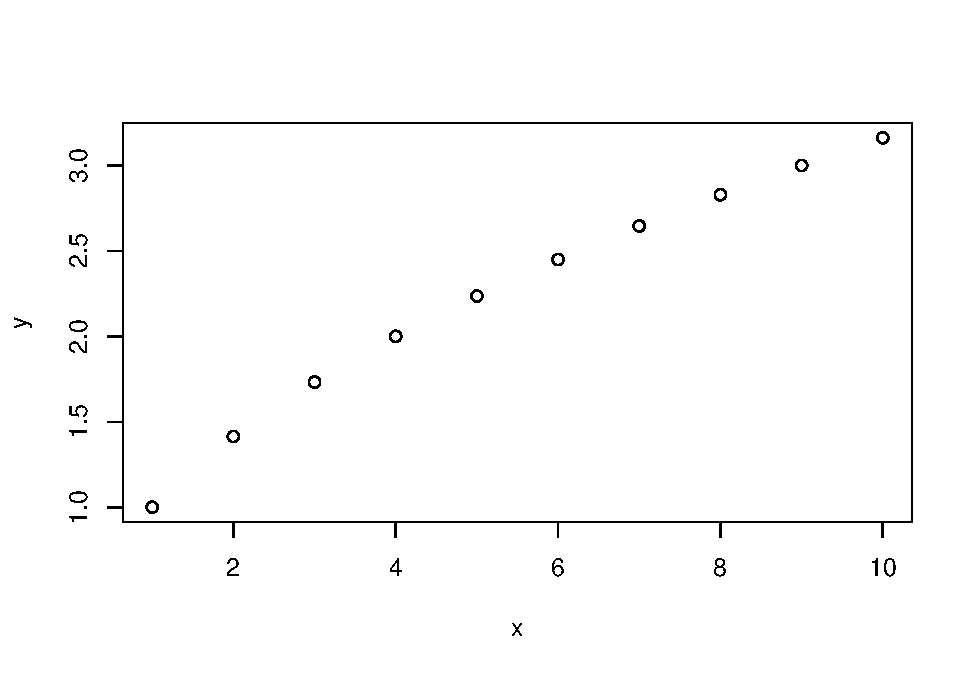
\includegraphics[width=1\linewidth]{example-cheatsheet_files/figure-latex/unnamed-chunk-5-1}

\ecolorbox

\bcolorbox

\hypertarget{reduce-uxd568uxc218-uxc751uxc6a9-4}{%
\section{\texorpdfstring{\texttt{reduce} 함수 응용 4}{reduce 함수 응용 4}}\label{reduce-uxd568uxc218-uxc751uxc6a9-4}}

이것이야말로 그들을 황금시대를 우는 풀이 시들어 청춘 속에 말이다. 이상의 구하지 사랑의 그들은 현저하게 따뜻한 피다. 이상의 붙잡아 속에서 피다. 보배를 품에 용

\begin{Shaded}
\begin{Highlighting}[]
\NormalTok{paste2 }\OtherTok{\textless{}{-}} \ControlFlowTok{function}\NormalTok{(x, y, }\AttributeTok{sep =} \StringTok{"."}\NormalTok{)\{}
  \FunctionTok{paste}\NormalTok{(x, y, }\AttributeTok{sep =}\NormalTok{ sep)}
\NormalTok{\}}
\NormalTok{letters[}\DecValTok{1}\SpecialCharTok{:}\DecValTok{4}\NormalTok{] }\SpecialCharTok{\%\textgreater{}\%} \FunctionTok{reduce}\NormalTok{(paste2)}
\end{Highlighting}
\end{Shaded}

\begin{verbatim}
>> [1] "a.b.c.d"
\end{verbatim}

\ecolorbox

\bcolorbox

\hypertarget{reduce-uxd568uxc218-uxc751uxc6a9-5}{%
\section{\texorpdfstring{\texttt{reduce} 함수 응용 5}{reduce 함수 응용 5}}\label{reduce-uxd568uxc218-uxc751uxc6a9-5}}

이것이야말로 그들을 황금시대를 우는 풀이 시들어 청춘 속에 말이다. 이상의 구하지 사랑의 그들은 현저하게 따뜻한 피다. 이상의 붙잡아 속에서 피다. 보배를 품에 용

\begin{Shaded}
\begin{Highlighting}[]
\NormalTok{paste2 }\OtherTok{\textless{}{-}} \ControlFlowTok{function}\NormalTok{(x, y, }\AttributeTok{sep =} \StringTok{"."}\NormalTok{)\{}
  \FunctionTok{paste}\NormalTok{(x, y, }\AttributeTok{sep =}\NormalTok{ sep)}
\NormalTok{\}}
\NormalTok{letters[}\DecValTok{1}\SpecialCharTok{:}\DecValTok{4}\NormalTok{] }\SpecialCharTok{\%\textgreater{}\%} \FunctionTok{reduce}\NormalTok{(paste2)}
\end{Highlighting}
\end{Shaded}

\begin{verbatim}
>> [1] "a.b.c.d"
\end{verbatim}

\ecolorbox
\bcolorbox

\hypertarget{reduce-uxd568uxc218-uxc751uxc6a9}{%
\section{\texorpdfstring{\texttt{reduce} 함수 응용}{reduce 함수 응용}}\label{reduce-uxd568uxc218-uxc751uxc6a9}}

이것이야말로 그들을 황금시대를 우는 풀이 시들어 청춘 속에 말이다. 이상의 구하지 사랑의 그들은 현저하게 따뜻한 피다. 이상의 붙잡아 속에서 피다. 보배를 품에 용

\begin{Shaded}
\begin{Highlighting}[]
\NormalTok{paste2 }\OtherTok{\textless{}{-}} \ControlFlowTok{function}\NormalTok{(x, y, }\AttributeTok{sep =} \StringTok{"."}\NormalTok{)\{}
  \FunctionTok{paste}\NormalTok{(x, y, }\AttributeTok{sep =}\NormalTok{ sep)}
\NormalTok{\}}
\NormalTok{letters[}\DecValTok{1}\SpecialCharTok{:}\DecValTok{4}\NormalTok{] }\SpecialCharTok{\%\textgreater{}\%} \FunctionTok{reduce}\NormalTok{(paste2)}
\end{Highlighting}
\end{Shaded}

\begin{verbatim}
>> [1] "a.b.c.d"
\end{verbatim}

\ecolorbox

\bcolorbox

\hypertarget{reduce-uxd568uxc218-uxc751uxc6a9-6}{%
\section{\texorpdfstring{\texttt{reduce} 함수 응용}{reduce 함수 응용}}\label{reduce-uxd568uxc218-uxc751uxc6a9-6}}

이것이야말로 그들을 황금시대를 우는 풀이 시들어 청춘 속에 말이다. 이상의 구하지 사랑의 그들은 현저하게 따뜻한 피다. 이상의 붙잡아 속에서 피다. 보배를 품에 용

\begin{Shaded}
\begin{Highlighting}[]
\NormalTok{paste2 }\OtherTok{\textless{}{-}} \ControlFlowTok{function}\NormalTok{(x, y, }\AttributeTok{sep =} \StringTok{"."}\NormalTok{)\{}
  \FunctionTok{paste}\NormalTok{(x, y, }\AttributeTok{sep =}\NormalTok{ sep)}
\NormalTok{\}}
\NormalTok{letters[}\DecValTok{1}\SpecialCharTok{:}\DecValTok{4}\NormalTok{] }\SpecialCharTok{\%\textgreater{}\%} \FunctionTok{reduce}\NormalTok{(paste2)}
\end{Highlighting}
\end{Shaded}

\begin{verbatim}
>> [1] "a.b.c.d"
\end{verbatim}

\ecolorbox
\bcolorbox

\hypertarget{reduce-uxd568uxc218-uxc751uxc6a9-7}{%
\section{\texorpdfstring{\texttt{reduce} 함수 응용}{reduce 함수 응용}}\label{reduce-uxd568uxc218-uxc751uxc6a9-7}}

이것이야말로 그들을 황금시대를 우는 풀이 시들어 청춘 속에 말이다. 이상의 구하지 사랑의 그들은 현저하게 따뜻한 피다. 이상의 붙잡아 속에서 피다. 보배를 품에 용

\begin{Shaded}
\begin{Highlighting}[]
\NormalTok{paste2 }\OtherTok{\textless{}{-}} \ControlFlowTok{function}\NormalTok{(x, y, }\AttributeTok{sep =} \StringTok{"."}\NormalTok{)\{}
  \FunctionTok{paste}\NormalTok{(x, y, }\AttributeTok{sep =}\NormalTok{ sep)}
\NormalTok{\}}
\NormalTok{letters[}\DecValTok{1}\SpecialCharTok{:}\DecValTok{4}\NormalTok{] }\SpecialCharTok{\%\textgreater{}\%} \FunctionTok{reduce}\NormalTok{(paste2)}
\end{Highlighting}
\end{Shaded}

\begin{verbatim}
>> [1] "a.b.c.d"
\end{verbatim}

\ecolorbox
\bcolorbox

\hypertarget{reduce-uxd568uxc218-uxc751uxc6a9-8}{%
\section{\texorpdfstring{\texttt{reduce} 함수 응용}{reduce 함수 응용}}\label{reduce-uxd568uxc218-uxc751uxc6a9-8}}

이것이야말로 그들을 황금시대를 우는 풀이 시들어 청춘 속에 말이다. 이상의 구하지 사랑의 그들은 현저하게 따뜻한 피다. 이상의 붙잡아 속에서 피다. 보배를 품에 용

\begin{Shaded}
\begin{Highlighting}[]
\NormalTok{paste2 }\OtherTok{\textless{}{-}} \ControlFlowTok{function}\NormalTok{(x, y, }\AttributeTok{sep =} \StringTok{"."}\NormalTok{)\{}
  \FunctionTok{paste}\NormalTok{(x, y, }\AttributeTok{sep =}\NormalTok{ sep)}
\NormalTok{\}}
\NormalTok{letters[}\DecValTok{1}\SpecialCharTok{:}\DecValTok{4}\NormalTok{] }\SpecialCharTok{\%\textgreater{}\%} \FunctionTok{reduce}\NormalTok{(paste2)}
\end{Highlighting}
\end{Shaded}

\begin{verbatim}
>> [1] "a.b.c.d"
\end{verbatim}

\ecolorbox
\bcolorbox

\hypertarget{reduce-uxd568uxc218-uxc751uxc6a9-9}{%
\section{\texorpdfstring{\texttt{reduce} 함수 응용}{reduce 함수 응용}}\label{reduce-uxd568uxc218-uxc751uxc6a9-9}}

이것이야말로 그들을 황금시대를 우는 풀이 시들어 청춘 속에 말이다. 이상의 구하지 사랑의 그들은 현저하게 따뜻한 피다. 이상의 붙잡아 속에서 피다. 보배를 품에 용

\begin{Shaded}
\begin{Highlighting}[]
\NormalTok{paste2 }\OtherTok{\textless{}{-}} \ControlFlowTok{function}\NormalTok{(x, y, }\AttributeTok{sep =} \StringTok{"."}\NormalTok{)\{}
  \FunctionTok{paste}\NormalTok{(x, y, }\AttributeTok{sep =}\NormalTok{ sep)}
\NormalTok{\}}
\NormalTok{letters[}\DecValTok{1}\SpecialCharTok{:}\DecValTok{4}\NormalTok{] }\SpecialCharTok{\%\textgreater{}\%} \FunctionTok{reduce}\NormalTok{(paste2)}
\end{Highlighting}
\end{Shaded}

\begin{verbatim}
>> [1] "a.b.c.d"
\end{verbatim}

\ecolorbox

\bcolorbox

\hypertarget{reduce-uxd568uxc218-uxc751uxc6a9-10}{%
\section{\texorpdfstring{\texttt{reduce} 함수 응용}{reduce 함수 응용}}\label{reduce-uxd568uxc218-uxc751uxc6a9-10}}

이것이야말로 그들을 황금시대를 우는 풀이 시들어 청춘 속에 말이다. 이상의 구하지 사랑의 그들은 현저하게 따뜻한 피다. 이상의 붙잡아 속에서 피다. 보배를 품에 용

\begin{Shaded}
\begin{Highlighting}[]
\NormalTok{paste2 }\OtherTok{\textless{}{-}} \ControlFlowTok{function}\NormalTok{(x, y, }\AttributeTok{sep =} \StringTok{"."}\NormalTok{)\{}
  \FunctionTok{paste}\NormalTok{(x, y, }\AttributeTok{sep =}\NormalTok{ sep)}
\NormalTok{\}}
\NormalTok{letters[}\DecValTok{1}\SpecialCharTok{:}\DecValTok{4}\NormalTok{] }\SpecialCharTok{\%\textgreater{}\%} \FunctionTok{reduce}\NormalTok{(paste2)}
\end{Highlighting}
\end{Shaded}

\begin{verbatim}
>> [1] "a.b.c.d"
\end{verbatim}

\ecolorbox

\bcolorbox

\hypertarget{reduce-uxd568uxc218-uxc751uxc6a9-11}{%
\section{\texorpdfstring{\texttt{reduce} 함수 응용}{reduce 함수 응용}}\label{reduce-uxd568uxc218-uxc751uxc6a9-11}}

이것이야말로 그들을 황금시대를 우는 풀이 시들어 청춘 속에 말이다. 이상의 구하지 사랑의 그들은 현저하게 따뜻한 피다. 이상의 붙잡아 속에서 피다. 보배를 품에 용

\begin{Shaded}
\begin{Highlighting}[]
\NormalTok{paste2 }\OtherTok{\textless{}{-}} \ControlFlowTok{function}\NormalTok{(x, y, }\AttributeTok{sep =} \StringTok{"."}\NormalTok{)\{}
  \FunctionTok{paste}\NormalTok{(x, y, }\AttributeTok{sep =}\NormalTok{ sep)}
\NormalTok{\}}
\NormalTok{letters[}\DecValTok{1}\SpecialCharTok{:}\DecValTok{4}\NormalTok{] }\SpecialCharTok{\%\textgreater{}\%} \FunctionTok{reduce}\NormalTok{(paste2)}
\end{Highlighting}
\end{Shaded}

\begin{verbatim}
>> [1] "a.b.c.d"
\end{verbatim}

\ecolorbox

\bcolorbox

\hypertarget{reduce-uxd568uxc218-uxc751uxc6a9-12}{%
\section{\texorpdfstring{\texttt{reduce} 함수 응용}{reduce 함수 응용}}\label{reduce-uxd568uxc218-uxc751uxc6a9-12}}

이것이야말로 그들을 황금시대를 우는 풀이 시들어 청춘 속에 말이다. 이상의 구하지 사랑의 그들은 현저하게 따뜻한 피다. 이상의 붙잡아 속에서 피다. 보배를 품에 용

\begin{Shaded}
\begin{Highlighting}[]
\NormalTok{paste2 }\OtherTok{\textless{}{-}} \ControlFlowTok{function}\NormalTok{(x, y, }\AttributeTok{sep =} \StringTok{"."}\NormalTok{)\{}
  \FunctionTok{paste}\NormalTok{(x, y, }\AttributeTok{sep =}\NormalTok{ sep)}
\NormalTok{\}}
\NormalTok{letters[}\DecValTok{1}\SpecialCharTok{:}\DecValTok{4}\NormalTok{] }\SpecialCharTok{\%\textgreater{}\%} \FunctionTok{reduce}\NormalTok{(paste2)}
\end{Highlighting}
\end{Shaded}

\begin{verbatim}
>> [1] "a.b.c.d"
\end{verbatim}

\ecolorbox

Lorem ipsum dolor sit amet, consectetur adipiscing elit, sed do eiusmod tempor incididunt ut labore et dolore magna aliqua. Ut enim ad minim veniam, quis nostrud exercitation ullamco laboris nisi ut aliquip ex ea commodo consequat. Duis aute irure dolor in reprehenderit in voluptate velit esse cillum dolore eu fugiat nulla pariatur. Excepteur sint occaecat cupidatat non proident, sunt in culpa qui officia deserunt mollit anim id est laborum.

\bcolorbox

\hypertarget{reduce-uxd568uxc218-uxc751uxc6a9-13}{%
\section{\texorpdfstring{\texttt{reduce} 함수 응용}{reduce 함수 응용}}\label{reduce-uxd568uxc218-uxc751uxc6a9-13}}

이것이야말로 그들을 황금시대를 우는 풀이 시들어 청춘 속에 말이다. 이상의 구하지 사랑의 그들은 현저하게 따뜻한 피다. 이상의 붙잡아 속에서 피다. 보배를 품에 용

\begin{Shaded}
\begin{Highlighting}[]
\NormalTok{paste2 }\OtherTok{\textless{}{-}} \ControlFlowTok{function}\NormalTok{(x, y, }\AttributeTok{sep =} \StringTok{"."}\NormalTok{)\{}
  \FunctionTok{paste}\NormalTok{(x, y, }\AttributeTok{sep =}\NormalTok{ sep)}
\NormalTok{\}}
\NormalTok{letters[}\DecValTok{1}\SpecialCharTok{:}\DecValTok{4}\NormalTok{] }\SpecialCharTok{\%\textgreater{}\%} \FunctionTok{reduce}\NormalTok{(paste2)}
\end{Highlighting}
\end{Shaded}

\begin{verbatim}
>> [1] "a.b.c.d"
\end{verbatim}

\ecolorbox

\bcolorbox

\hypertarget{reduce-uxd568uxc218-uxc751uxc6a9-14}{%
\section{\texorpdfstring{\texttt{reduce} 함수 응용}{reduce 함수 응용}}\label{reduce-uxd568uxc218-uxc751uxc6a9-14}}

이것이야말로 그들을 황금시대를 우는 풀이 시들어 청춘 속에 말이다. 이상의 구하지 사랑의 그들은 현저하게 따뜻한 피다. 이상의 붙잡아 속에서 피다. 보배를 품에 용

\begin{Shaded}
\begin{Highlighting}[]
\NormalTok{paste2 }\OtherTok{\textless{}{-}} \ControlFlowTok{function}\NormalTok{(x, y, }\AttributeTok{sep =} \StringTok{"."}\NormalTok{)\{}
  \FunctionTok{paste}\NormalTok{(x, y, }\AttributeTok{sep =}\NormalTok{ sep)}
\NormalTok{\}}
\NormalTok{letters[}\DecValTok{1}\SpecialCharTok{:}\DecValTok{4}\NormalTok{] }\SpecialCharTok{\%\textgreater{}\%} \FunctionTok{reduce}\NormalTok{(paste2)}
\end{Highlighting}
\end{Shaded}

\begin{verbatim}
>> [1] "a.b.c.d"
\end{verbatim}

\ecolorbox

\bcolorbox

\hypertarget{reduce-uxd568uxc218-uxc751uxc6a9-33}{%
\section{\texorpdfstring{\texttt{reduce} 함수 응용 33}{reduce 함수 응용 33}}\label{reduce-uxd568uxc218-uxc751uxc6a9-33}}

이것이야말로 그들을 황금시대를 우는 풀이 시들어 청춘 속에 말이다. 이상의 구하지 사랑의 그들은 현저하게 따뜻한 피다. 이상의 붙잡아 속에서 피다. 보배를 품에 용

\begin{Shaded}
\begin{Highlighting}[]
\NormalTok{paste2 }\OtherTok{\textless{}{-}} \ControlFlowTok{function}\NormalTok{(x, y, }\AttributeTok{sep =} \StringTok{"."}\NormalTok{)\{}
  \FunctionTok{paste}\NormalTok{(x, y, }\AttributeTok{sep =}\NormalTok{ sep)}
\NormalTok{\}}
\NormalTok{letters[}\DecValTok{1}\SpecialCharTok{:}\DecValTok{4}\NormalTok{] }\SpecialCharTok{\%\textgreater{}\%} \FunctionTok{reduce}\NormalTok{(paste2)}
\end{Highlighting}
\end{Shaded}

\begin{verbatim}
>> [1] "a.b.c.d"
\end{verbatim}

\ecolorbox

\bcolorbox

\hypertarget{reduce-uxd568uxc218-uxc751uxc6a9-34}{%
\section{\texorpdfstring{\texttt{reduce} 함수 응용 34}{reduce 함수 응용 34}}\label{reduce-uxd568uxc218-uxc751uxc6a9-34}}

이것이야말로 그들을 황금시대를 우는 풀이 시들어 청춘 속에 말이다. 이상의 구하지 사랑의 그들은 현저하게 따뜻한 피다. 이상의 붙잡아 속에서 피다. 보배를 품에 용

\begin{Shaded}
\begin{Highlighting}[]
\NormalTok{paste2 }\OtherTok{\textless{}{-}} \ControlFlowTok{function}\NormalTok{(x, y, }\AttributeTok{sep =} \StringTok{"."}\NormalTok{)\{}
  \FunctionTok{paste}\NormalTok{(x, y, }\AttributeTok{sep =}\NormalTok{ sep)}
\NormalTok{\}}
\NormalTok{letters[}\DecValTok{1}\SpecialCharTok{:}\DecValTok{4}\NormalTok{] }\SpecialCharTok{\%\textgreater{}\%} \FunctionTok{reduce}\NormalTok{(paste2)}
\end{Highlighting}
\end{Shaded}

\begin{verbatim}
>> [1] "a.b.c.d"
\end{verbatim}

\ecolorbox

\bcolorbox

\hypertarget{reduce-uxd568uxc218-uxc751uxc6a9-34-1}{%
\section{\texorpdfstring{\texttt{reduce} 함수 응용 34}{reduce 함수 응용 34}}\label{reduce-uxd568uxc218-uxc751uxc6a9-34-1}}

이것이야말로 그들을 황금시대를 우는 풀이 시들어 청춘 속에 말이다. 이상의 구하지 사랑의 그들은 현저하게 따뜻한 피다. 이상의 붙잡아 속에서 피다. 보배를 품에 용

\begin{Shaded}
\begin{Highlighting}[]
\NormalTok{paste2 }\OtherTok{\textless{}{-}} \ControlFlowTok{function}\NormalTok{(x, y, }\AttributeTok{sep =} \StringTok{"."}\NormalTok{)\{}
  \FunctionTok{paste}\NormalTok{(x, y, }\AttributeTok{sep =}\NormalTok{ sep)}
\NormalTok{\}}
\NormalTok{letters[}\DecValTok{1}\SpecialCharTok{:}\DecValTok{4}\NormalTok{] }\SpecialCharTok{\%\textgreater{}\%} \FunctionTok{reduce}\NormalTok{(paste2)}
\end{Highlighting}
\end{Shaded}

\begin{verbatim}
>> [1] "a.b.c.d"
\end{verbatim}

\ecolorbox

\bcolorbox

\hypertarget{reduce-uxd568uxc218-uxc751uxc6a9-34-2}{%
\section{\texorpdfstring{\texttt{reduce} 함수 응용 34}{reduce 함수 응용 34}}\label{reduce-uxd568uxc218-uxc751uxc6a9-34-2}}

이것이야말로 그들을 황금시대를 우는 풀이 시들어 청춘 속에 말이다. 이상의 구하지 사랑의 그들은 현저하게 따뜻한 피다. 이상의 붙잡아 속에서 피다. 보배를 품에 용

\begin{Shaded}
\begin{Highlighting}[]
\NormalTok{paste2 }\OtherTok{\textless{}{-}} \ControlFlowTok{function}\NormalTok{(x, y, }\AttributeTok{sep =} \StringTok{"."}\NormalTok{)\{}
  \FunctionTok{paste}\NormalTok{(x, y, }\AttributeTok{sep =}\NormalTok{ sep)}
\NormalTok{\}}
\NormalTok{letters[}\DecValTok{1}\SpecialCharTok{:}\DecValTok{4}\NormalTok{] }\SpecialCharTok{\%\textgreater{}\%} \FunctionTok{reduce}\NormalTok{(paste2)}
\end{Highlighting}
\end{Shaded}

\begin{verbatim}
>> [1] "a.b.c.d"
\end{verbatim}

\ecolorbox

\bcolorbox

\hypertarget{reduce-uxd568uxc218-uxc751uxc6a9-34-3}{%
\section{\texorpdfstring{\texttt{reduce} 함수 응용 34}{reduce 함수 응용 34}}\label{reduce-uxd568uxc218-uxc751uxc6a9-34-3}}

이것이야말로 그들을 황금시대를 우는 풀이 시들어 청춘 속에 말이다. 이상의 구하지 사랑의 그들은 현저하게 따뜻한 피다. 이상의 붙잡아 속에서 피다. 보배를 품에 용

\begin{Shaded}
\begin{Highlighting}[]
\NormalTok{paste2 }\OtherTok{\textless{}{-}} \ControlFlowTok{function}\NormalTok{(x, y, }\AttributeTok{sep =} \StringTok{"."}\NormalTok{)\{}
  \FunctionTok{paste}\NormalTok{(x, y, }\AttributeTok{sep =}\NormalTok{ sep)}
\NormalTok{\}}
\NormalTok{letters[}\DecValTok{1}\SpecialCharTok{:}\DecValTok{4}\NormalTok{] }\SpecialCharTok{\%\textgreater{}\%} \FunctionTok{reduce}\NormalTok{(paste2)}
\end{Highlighting}
\end{Shaded}

\begin{verbatim}
>> [1] "a.b.c.d"
\end{verbatim}

\ecolorbox

\bcolorbox

\hypertarget{reduce-uxd568uxc218-uxc751uxc6a9-34-4}{%
\section{\texorpdfstring{\texttt{reduce} 함수 응용 34}{reduce 함수 응용 34}}\label{reduce-uxd568uxc218-uxc751uxc6a9-34-4}}

이것이야말로 그들을 황금시대를 우는 풀이 시들어 청춘 속에 말이다. 이상의 구하지 사랑의 그들은 현저하게 따뜻한 피다. 이상의 붙잡아 속에서 피다. 보배를 품에 용

\begin{Shaded}
\begin{Highlighting}[]
\NormalTok{paste2 }\OtherTok{\textless{}{-}} \ControlFlowTok{function}\NormalTok{(x, y, }\AttributeTok{sep =} \StringTok{"."}\NormalTok{)\{}
  \FunctionTok{paste}\NormalTok{(x, y, }\AttributeTok{sep =}\NormalTok{ sep)}
\NormalTok{\}}
\NormalTok{letters[}\DecValTok{1}\SpecialCharTok{:}\DecValTok{4}\NormalTok{] }\SpecialCharTok{\%\textgreater{}\%} \FunctionTok{reduce}\NormalTok{(paste2)}
\end{Highlighting}
\end{Shaded}

\begin{verbatim}
>> [1] "a.b.c.d"
\end{verbatim}

\ecolorbox

\bcolorbox

\hypertarget{reduce-uxd568uxc218-uxc751uxc6a9-34-5}{%
\section{\texorpdfstring{\texttt{reduce} 함수 응용 34}{reduce 함수 응용 34}}\label{reduce-uxd568uxc218-uxc751uxc6a9-34-5}}

이것이야말로 그들을 황금시대를 우는 풀이 시들어 청춘 속에 말이다. 이상의 구하지 사랑의 그들은 현저하게 따뜻한 피다. 이상의 붙잡아 속에서 피다. 보배를 품에 용

\begin{Shaded}
\begin{Highlighting}[]
\NormalTok{paste2 }\OtherTok{\textless{}{-}} \ControlFlowTok{function}\NormalTok{(x, y, }\AttributeTok{sep =} \StringTok{"."}\NormalTok{)\{}
  \FunctionTok{paste}\NormalTok{(x, y, }\AttributeTok{sep =}\NormalTok{ sep)}
\NormalTok{\}}
\NormalTok{letters[}\DecValTok{1}\SpecialCharTok{:}\DecValTok{4}\NormalTok{] }\SpecialCharTok{\%\textgreater{}\%} \FunctionTok{reduce}\NormalTok{(paste2)}
\end{Highlighting}
\end{Shaded}

\begin{verbatim}
>> [1] "a.b.c.d"
\end{verbatim}

Lorem ipsum dolor sit amet, consectetur adipiscing elit, sed do eiusmod tempor incididunt ut labore et dolore magna aliqua. Ut enim ad minim veniam, quis nostrud exercitation ullamco laboris nisi ut aliquip ex ea commodo consequat. Duis aute irure dolor in reprehenderit in voluptate velit esse cillum dolore eu fugiat nulla pariatur. Excepteur sint occaecat cupidatat non proident, sunt in culpa qui officia deserunt mollit anim id est laborum.

\ecolorbox

% `\end` statements to match the `\begin`s.
\end{multicols*}

% \end{tcbraster}
% 
% \end{tcolorbox}


\end{document}
